\documentclass[15pt, mathserif]{beamer}

\usepackage[french]{babel}
\usepackage[T1]{fontenc}
\usepackage[utf8]{inputenc}
%\usepackage{esvect}
\usepackage{bm}
\usepackage{eurosym}
\usepackage{tikz}
\usepackage{pgf,tikz,pgfplots}
\pgfplotsset{compat=1.15}
\usepackage{mathrsfs}
\usetikzlibrary{arrows}
\usetikzlibrary{arrows.meta}

\usetikzlibrary{mindmap}
\usepackage{multicol}
\usepackage[tikz]{bclogo}
\usepackage{tkz-tab}
\usepackage{amsmath, tabu}
\usepackage{esvect} %\vv{AB} pour le vecteur AB

\DeclareMathOperator{\e}{e}

%% Tableau

\usepackage{makecell}
\setcellgapes{1pt}
\makegapedcells
\newcolumntype{R}[1]{>{\raggedleft\arraybackslash }b{#1}}
\newcolumntype{L}[1]{>{\raggedright\arraybackslash }b{#1}}
\newcolumntype{C}[1]{>{\centering\arraybackslash }b{#1}}


%pour avoir des parenthèses rondes dans le package fourier
\DeclareSymbolFont{cmoperators}   {OT1}{cmr} {m}{n}
\DeclareSymbolFont{cmlargesymbols}{OMX}{cmex}{m}{n}

\usefonttheme{professionalfonts} %permet d'enlever un bug avec fourier
\usepackage{fourier}
\DeclareMathDelimiter{(}{\mathopen} {cmoperators}{"28}{cmlargesymbols}{"00}
\DeclareMathDelimiter{)}{\mathclose}{cmoperators}{"29}{cmlargesymbols}{"01}

%Graphiques 

\usepackage{pgf,tikz,pgfplots}
\pgfplotsset{compat=1.15}
\usepackage{mathrsfs}
\usetikzlibrary{arrows}
\usetikzlibrary{mindmap}

%ensembles de nbres

\newcommand{\R}{\mathbb{R}}			%permet d'écrire le R "ensemble des réels"'
\newcommand{\N}{\mathbb{N}}			%permet d'écrire le N "ensemble des entiers naturels"
\newcommand{\Z}{\mathbb{Z}}			%permet d'écrire le Z "ensemble des entiers relatifs"
\newcommand{\Prem}{\mathbb{P}}	%permet d'écrire le P "ensemble des nombres premiers" (qui n'a pas marché avec le \P car il existe déjà)
\newcommand{\D}{\mathbb{D}}
\newcommand{\Df}{\mathcal{D}_f}
\newcommand{\Cf}{\mathcal{C}_f}

\newcommand{\Q}{\mathbb{Q}}


\newcommand{\st}[1]{$(#1_n)_{n \in \N}$}

\usetheme{Madrid}
\useoutertheme{miniframes} % Alternatively: miniframes, infolines, split
\useinnertheme{circles}
\definecolor{UBCblue}{rgb}{0.1, 0.25, 0.4} % UBC Blue (primary)
\definecolor{bordeaux}{RGB}{128,0,0}
\usecolortheme[named=UBCblue]{structure}

\usepackage{color} % J'aime bien définir mes couleurs
\definecolor{propcolor}{rgb}{0, 0.5, 1}
\definecolor{thcolor}{rgb}{0.6, 0.07, 0.07}
\colorlet{louis}{blue!70!green!60!white}
\colorlet{sakura}{pink!40!red}

\title{Activités Mentales}
\date{24 Août 2023}

\newcommand{\vco}[2]{\begin{pmatrix} #1 \\ #2 \end{pmatrix}} %Coordonnées de vecteur
\newenvironment{eq}{\begin{cases}\begin{tabu}{ccccc}}{\end{tabu}\end{cases}}
\newenvironment{eql}{\begin{cases}\begin{tabu}{cccccl}}{\end{tabu}\end{cases}}
\newenvironment{eqrl}{\begin{cases}\begin{tabu}{rl}}{\end{tabu}\end{cases}}

\newenvironment{Eq}{\begin{center}\begin{tabular}{rrcl}}{\end{tabular}\end{center}}
\newcommand{\ligneq}[2]{$\Longleftrightarrow$ & $#1$ & $=$ & $#2$ \\}
\newcommand{\Ligneq}[2]{ & $#1$ & $=$ & $#2$ \\}

\newenvironment{RPN}{\begin{center}\begin{tabular}{rrclcrcl}}{\end{tabular}\end{center}}
\newcommand{\Lignerpn}[4]{ & $#1$ & $=$ & $#2$ & ou & $#3$ & $=$ & $#4$ \\}
\newcommand{\lignerpn}[4]{$\Longleftrightarrow$ & $#1$ & $=$ & $#2$ & ou & $#3$ & $=$ & $#4$ \\}

\newenvironment{TRPN}{\begin{center}\begin{tabular}{rrclcrclcrcl}}{\end{tabular}\end{center}}
\newcommand{\Lignetrpn}[6]{ & $#1$ & $=$ & $#2$ & ou & $#3$ & $=$ & $#4$ & ou & $#5$ & $=$ & $#6$ \\}
\newcommand{\lignetrpn}[6]{$\Longleftrightarrow$ & $#1$ & $=$ & $#2$ & ou & $#3$ & $=$ & $#4$ & ou & $#5$ & $=$ & $#6$ \\}
\begin{document}

\begin{frame}
    \titlepage
\end{frame}

\begin{frame} 
	\frametitle{Question 1}
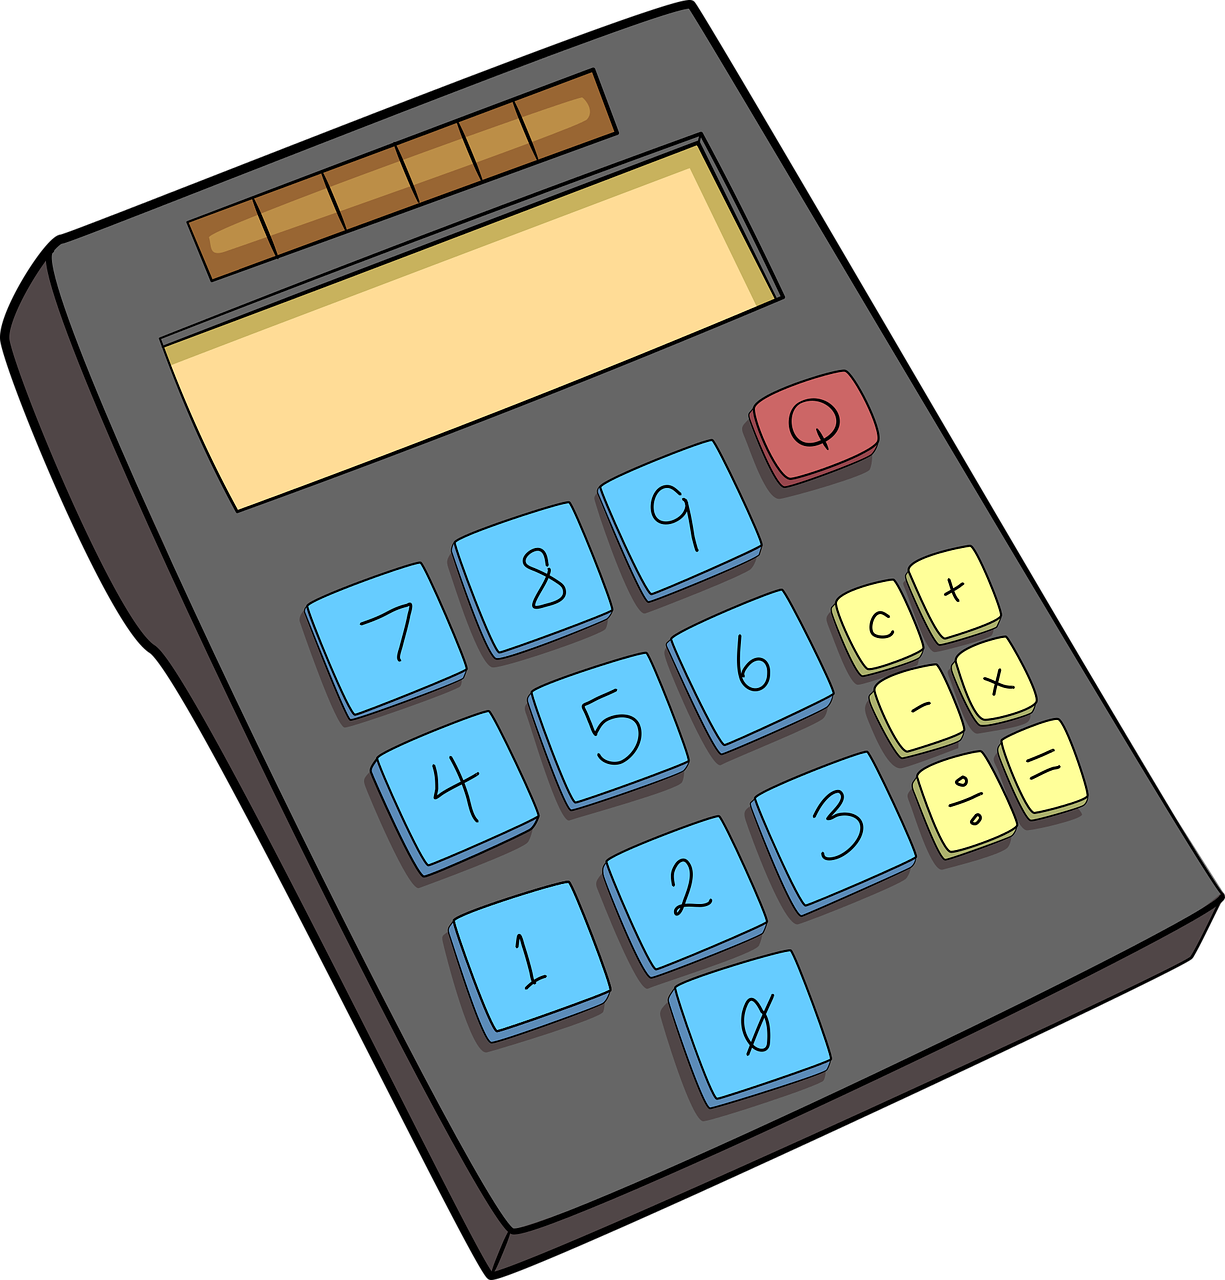
\includegraphics[scale=0.01]{calculatrice}  On considère le tableau suivant récapitulant les notes d'un élève au cours d'un trimestre. 
 
 \begin{center} 
 \begin{tabular}{|p{2cm}|p{0.5cm}|p{0.5cm}|p{0.5cm}|p{0.5cm}|p{0.5cm}|p{0.5cm}|p{0.5cm}|p{0.5cm}|} 
 \hline 
  \centering Devoir & \centering 1& \centering 2& \centering 3& \centering 4& \centering 5& \centering 6& \centering 7& \centering 8\tabularnewline  
 \hline 
 \centering Note (/20) & \centering 12& \centering 17& \centering 11& \centering 18& \centering 19& \centering 10& \centering 14& \centering 10\tabularnewline  
 \hline 
 \centering Coefficient & \centering 0.25& \centering 4& \centering 0.5& \centering 4& \centering 4& \centering 1.5& \centering 1.5& \centering 0.25\tabularnewline  
 \hline 
 \end{tabular} 
 \end{center}  
 
 Calculer la moyenne de cet élève. \end{frame}


\begin{frame} 
	\frametitle{Question 2}
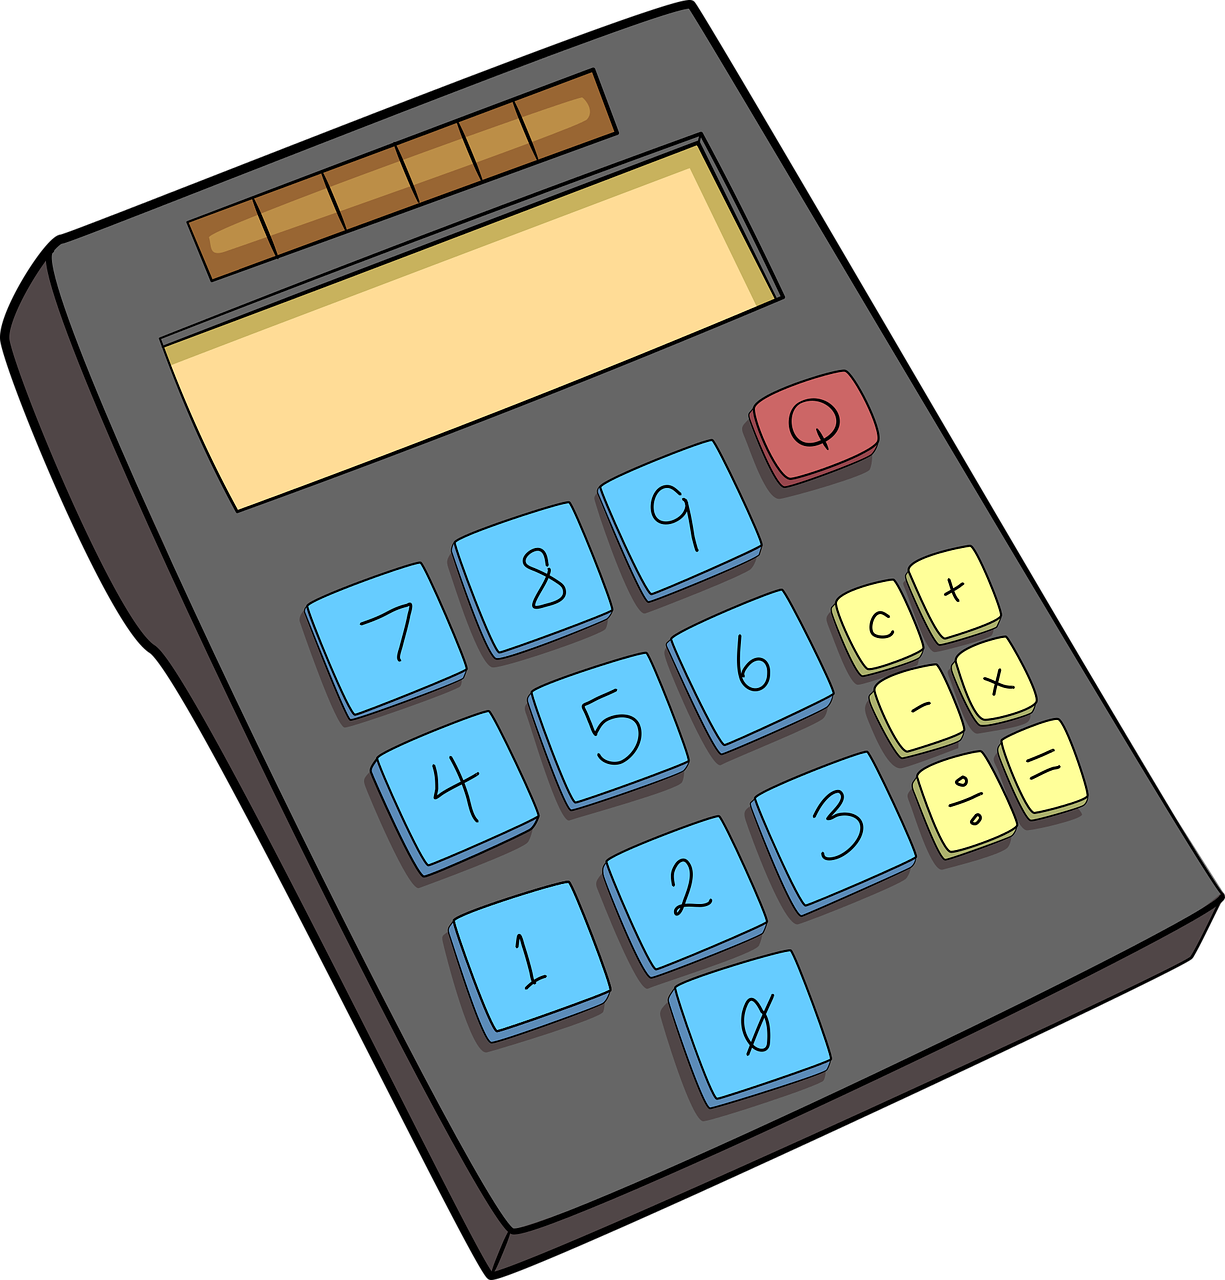
\includegraphics[scale=0.01]{calculatrice}  On considère le tableau suivant récapitulant les notes d'un élève au cours d'un trimestre. 
 
 \begin{center} 
 \begin{tabular}{|p{2cm}|p{0.5cm}|p{0.5cm}|p{0.5cm}|p{0.5cm}|p{0.5cm}|} 
 \hline 
  \centering Devoir & \centering 1& \centering 2& \centering 3& \centering 4& \centering 5\tabularnewline  
 \hline 
 \centering Note (/20) & \centering 16& \centering 8& \centering 20& \centering 6& \centering 16\tabularnewline  
 \hline 
 \centering Coefficient & \centering 0.5& \centering 4& \centering 0.25& \centering 0.5& \centering 4\tabularnewline  
 \hline 
 \end{tabular} 
 \end{center}  
 
 Calculer la moyenne de cet élève. \end{frame}


\begin{frame} 
	\frametitle{Question 3}
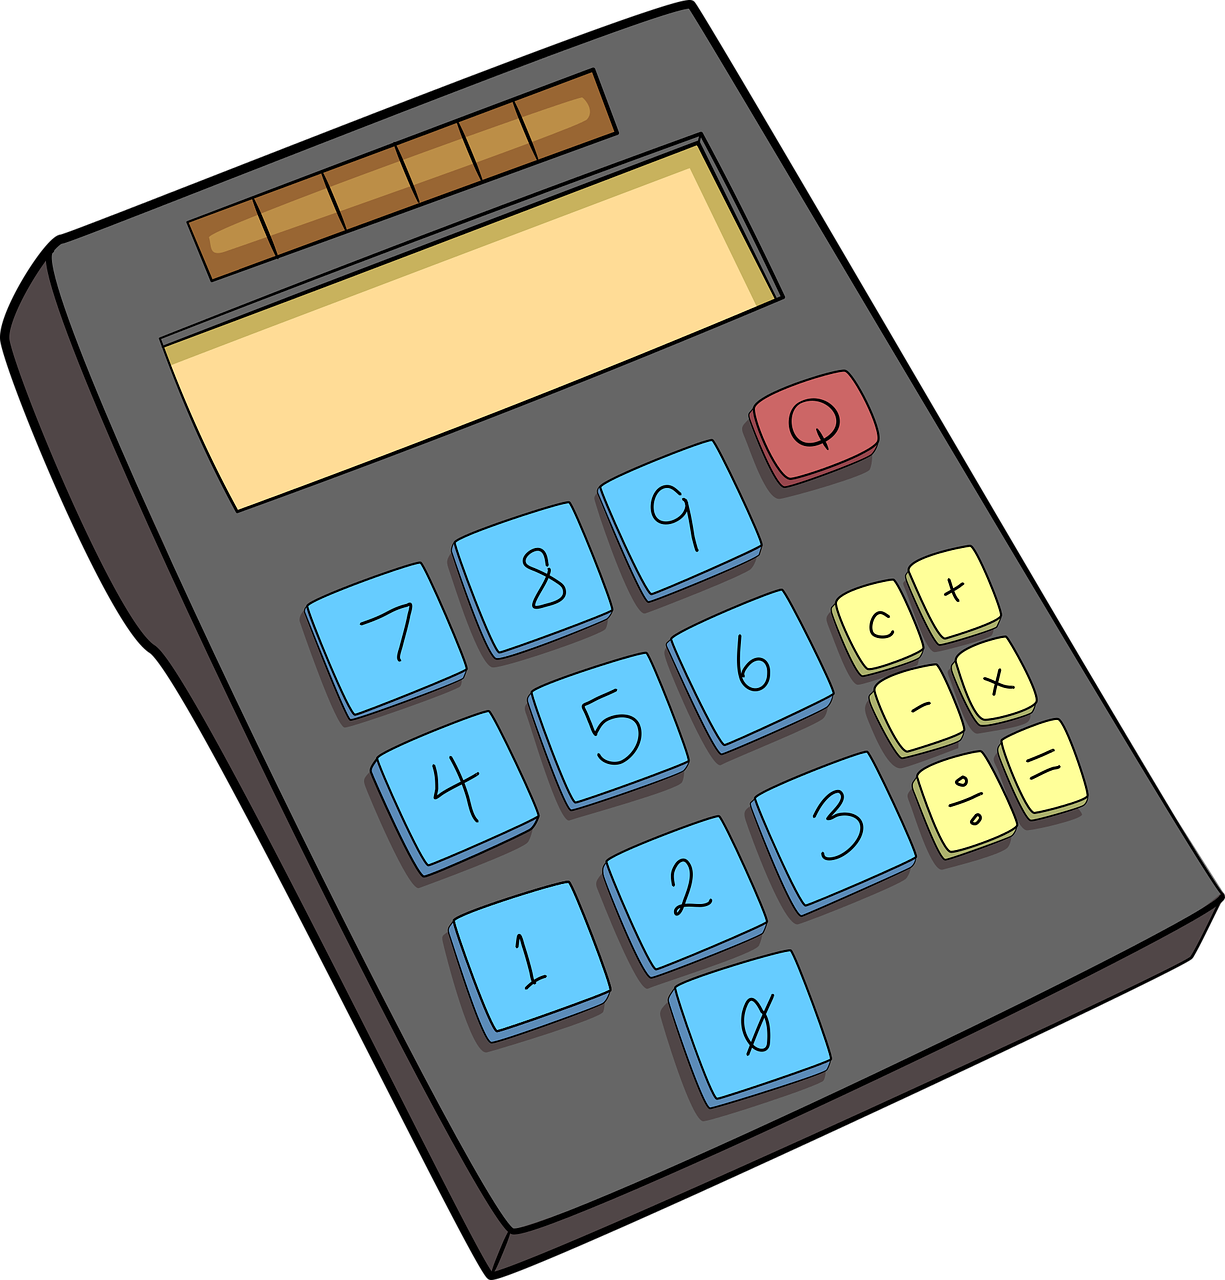
\includegraphics[scale=0.01]{calculatrice}  On considère le tableau suivant récapitulant les notes d'un élève au cours d'un trimestre. 
 
 \begin{center} 
 \begin{tabular}{|p{2cm}|p{0.5cm}|p{0.5cm}|p{0.5cm}|p{0.5cm}|p{0.5cm}|p{0.5cm}|} 
 \hline 
  \centering Devoir & \centering 1& \centering 2& \centering 3& \centering 4& \centering 5& \centering 6\tabularnewline  
 \hline 
 \centering Note (/20) & \centering 15& \centering 19& \centering 18& \centering 8& \centering 18& \centering 13\tabularnewline  
 \hline 
 \centering Coefficient & \centering 1.5& \centering 0.5& \centering 1& \centering 1& \centering 1& \centering 0.5\tabularnewline  
 \hline 
 \end{tabular} 
 \end{center}  
 
 Calculer la moyenne de cet élève. \end{frame}


\begin{frame} 
	\frametitle{Question 4}
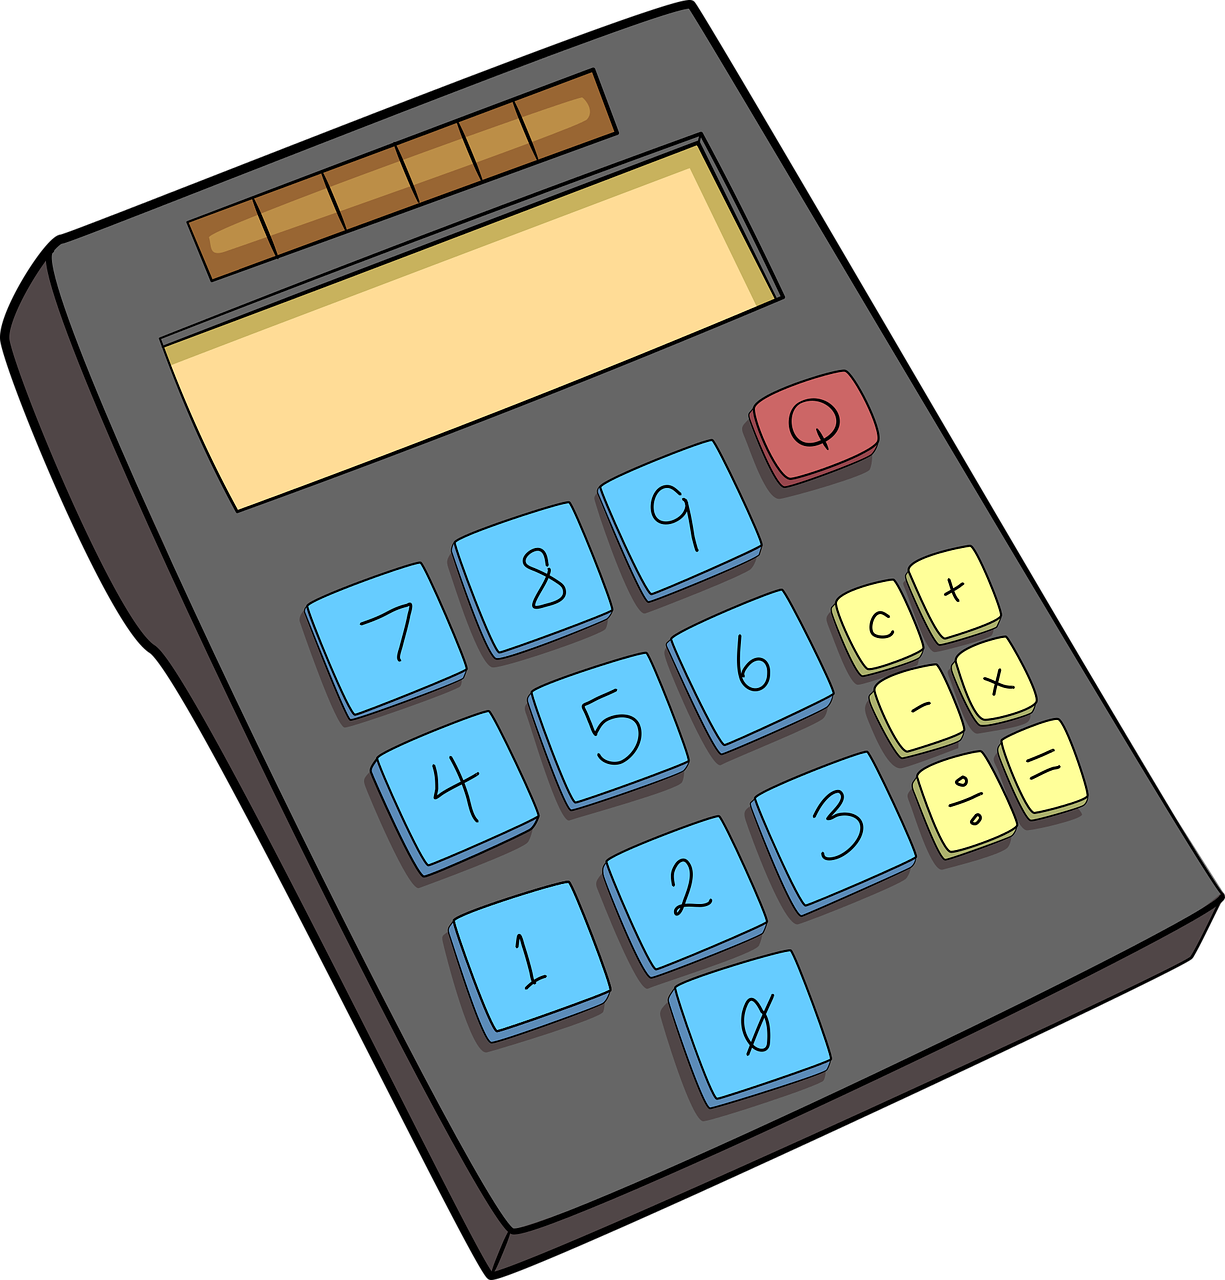
\includegraphics[scale=0.01]{calculatrice}  On considère le tableau suivant récapitulant les notes d'un élève au cours d'un trimestre. 
 
 \begin{center} 
 \begin{tabular}{|p{2cm}|p{0.5cm}|p{0.5cm}|p{0.5cm}|p{0.5cm}|} 
 \hline 
  \centering Devoir & \centering 1& \centering 2& \centering 3& \centering 4\tabularnewline  
 \hline 
 \centering Note (/20) & \centering 6& \centering 20& \centering 18& \centering 17\tabularnewline  
 \hline 
 \centering Coefficient & \centering 0.25& \centering 4& \centering 4& \centering 2\tabularnewline  
 \hline 
 \end{tabular} 
 \end{center}  
 
 Calculer la moyenne de cet élève. \end{frame}


\begin{frame} 
	\frametitle{Question 5}
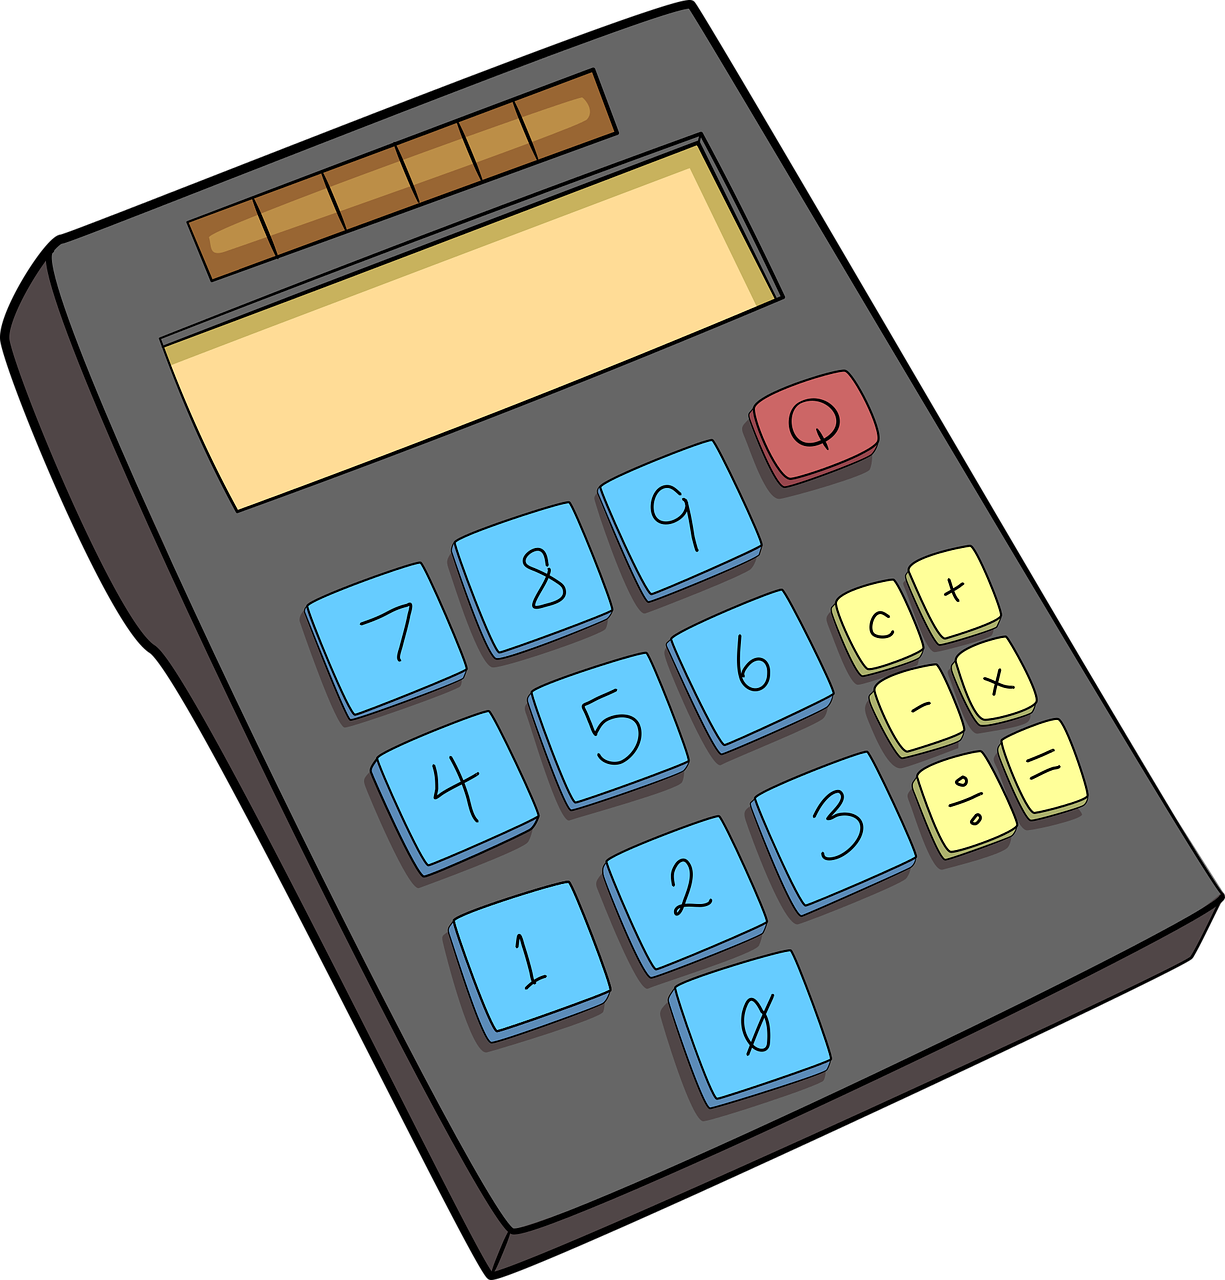
\includegraphics[scale=0.01]{calculatrice}  On considère le tableau suivant récapitulant les notes d'un élève au cours d'un trimestre. 
 
 \begin{center} 
 \begin{tabular}{|p{2cm}|p{0.5cm}|p{0.5cm}|p{0.5cm}|p{0.5cm}|p{0.5cm}|} 
 \hline 
  \centering Devoir & \centering 1& \centering 2& \centering 3& \centering 4& \centering 5\tabularnewline  
 \hline 
 \centering Note (/20) & \centering 8& \centering 7& \centering 11& \centering 10& \centering 6\tabularnewline  
 \hline 
 \centering Coefficient & \centering 1& \centering 2& \centering 4& \centering 0.25& \centering 0.25\tabularnewline  
 \hline 
 \end{tabular} 
 \end{center}  
 
 Calculer la moyenne de cet élève. \end{frame}


\begin{frame}
\vspace{-10mm}
	\frametitle{Correction 1}
 \begin{center} 
 \begin{tabular}{|p{2cm}|p{0.5cm}|p{0.5cm}|p{0.5cm}|p{0.5cm}|p{0.5cm}|p{0.5cm}|p{0.5cm}|p{0.5cm}|} 
 \hline 
  \centering Devoir & \centering 1& \centering 2& \centering 3& \centering 4& \centering 5& \centering 6& \centering 7& \centering 8\tabularnewline  
 \hline 
 \centering Note (/20) & \centering 12& \centering 17& \centering 11& \centering 18& \centering 19& \centering 10& \centering 14& \centering 10\tabularnewline  
 \hline 
 \centering Coefficient & \centering 0.25& \centering 4& \centering 0.5& \centering 4& \centering 4& \centering 1.5& \centering 1.5& \centering 0.25\tabularnewline  
 \hline 
 \end{tabular} 
 \end{center}  En notant $m$ la moyenne, on a \begin{align*} 
 m&= \dfrac{12\times 0.25+17\times 4+11\times 0.5+18\times 4+19\times 4+10\times 1.5+14\times 1.5+10\times 0.25}{0.25+4+0.5+4+4+1.5+1.5+0.25}\\ 
 &=\dfrac{3.0+68+5.5+72+76+15.0+21.0+2.5}{16.0} \\ 
 &\simeq16.44\end{align*}\end{frame}


\begin{frame}
\vspace{-10mm}
	\frametitle{Correction 2}
 \begin{center} 
 \begin{tabular}{|p{2cm}|p{0.5cm}|p{0.5cm}|p{0.5cm}|p{0.5cm}|p{0.5cm}|} 
 \hline 
  \centering Devoir & \centering 1& \centering 2& \centering 3& \centering 4& \centering 5\tabularnewline  
 \hline 
 \centering Note (/20) & \centering 16& \centering 8& \centering 20& \centering 6& \centering 16\tabularnewline  
 \hline 
 \centering Coefficient & \centering 0.5& \centering 4& \centering 0.25& \centering 0.5& \centering 4\tabularnewline  
 \hline 
 \end{tabular} 
 \end{center}  En notant $m$ la moyenne, on a \begin{align*} 
 m&= \dfrac{16\times 0.5+8\times 4+20\times 0.25+6\times 0.5+16\times 4}{0.5+4+0.25+0.5+4}\\ 
 &=\dfrac{8.0+32+5.0+3.0+64}{9.25} \\ 
 &\simeq12.11\end{align*}\end{frame}


\begin{frame}
\vspace{-10mm}
	\frametitle{Correction 3}
 \begin{center} 
 \begin{tabular}{|p{2cm}|p{0.5cm}|p{0.5cm}|p{0.5cm}|p{0.5cm}|p{0.5cm}|p{0.5cm}|} 
 \hline 
  \centering Devoir & \centering 1& \centering 2& \centering 3& \centering 4& \centering 5& \centering 6\tabularnewline  
 \hline 
 \centering Note (/20) & \centering 15& \centering 19& \centering 18& \centering 8& \centering 18& \centering 13\tabularnewline  
 \hline 
 \centering Coefficient & \centering 1.5& \centering 0.5& \centering 1& \centering 1& \centering 1& \centering 0.5\tabularnewline  
 \hline 
 \end{tabular} 
 \end{center}  En notant $m$ la moyenne, on a \begin{align*} 
 m&= \dfrac{15\times 1.5+19\times 0.5+18\times 1+8\times 1+18\times 1+13\times 0.5}{1.5+0.5+1+1+1+0.5}\\ 
 &=\dfrac{22.5+9.5+18+8+18+6.5}{5.5} \\ 
 &\simeq15.0\end{align*}\end{frame}


\begin{frame}
\vspace{-10mm}
	\frametitle{Correction 4}
 \begin{center} 
 \begin{tabular}{|p{2cm}|p{0.5cm}|p{0.5cm}|p{0.5cm}|p{0.5cm}|} 
 \hline 
  \centering Devoir & \centering 1& \centering 2& \centering 3& \centering 4\tabularnewline  
 \hline 
 \centering Note (/20) & \centering 6& \centering 20& \centering 18& \centering 17\tabularnewline  
 \hline 
 \centering Coefficient & \centering 0.25& \centering 4& \centering 4& \centering 2\tabularnewline  
 \hline 
 \end{tabular} 
 \end{center}  En notant $m$ la moyenne, on a \begin{align*} 
 m&= \dfrac{6\times 0.25+20\times 4+18\times 4+17\times 2}{0.25+4+4+2}\\ 
 &=\dfrac{1.5+80+72+34}{10.25} \\ 
 &\simeq18.29\end{align*}\end{frame}


\begin{frame}
\vspace{-10mm}
	\frametitle{Correction 5}
 \begin{center} 
 \begin{tabular}{|p{2cm}|p{0.5cm}|p{0.5cm}|p{0.5cm}|p{0.5cm}|p{0.5cm}|} 
 \hline 
  \centering Devoir & \centering 1& \centering 2& \centering 3& \centering 4& \centering 5\tabularnewline  
 \hline 
 \centering Note (/20) & \centering 8& \centering 7& \centering 11& \centering 10& \centering 6\tabularnewline  
 \hline 
 \centering Coefficient & \centering 1& \centering 2& \centering 4& \centering 0.25& \centering 0.25\tabularnewline  
 \hline 
 \end{tabular} 
 \end{center}  En notant $m$ la moyenne, on a \begin{align*} 
 m&= \dfrac{8\times 1+7\times 2+11\times 4+10\times 0.25+6\times 0.25}{1+2+4+0.25+0.25}\\ 
 &=\dfrac{8+14+44+2.5+1.5}{7.5} \\ 
 &\simeq9.33\end{align*}\end{frame}




\end{document}